% Generado desde docs/INFORME.md. Editar libremente.

\section{2. Dominio y límites de los microservicios}

\begin{figure}[H]
\centering
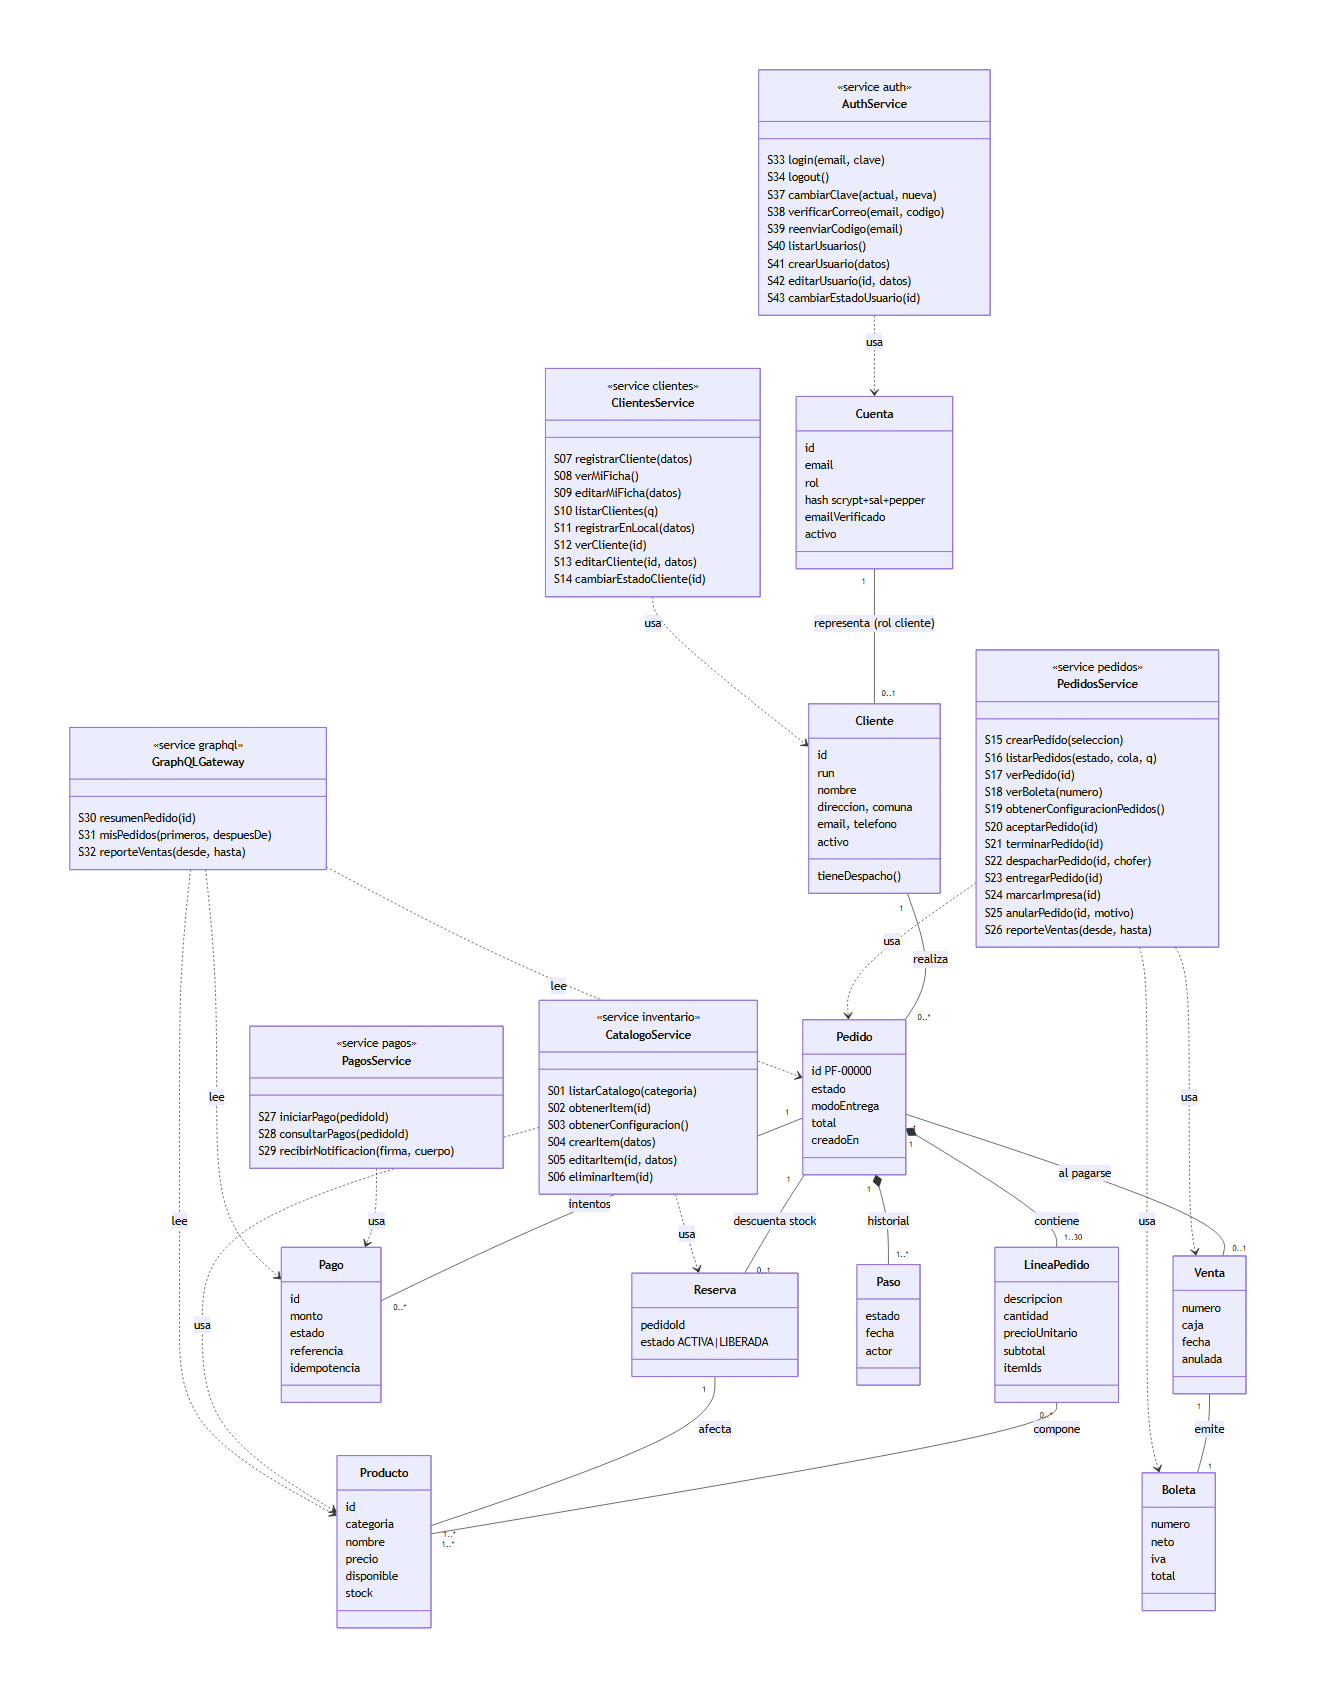
\includegraphics[width=\linewidth,height=0.8\textheight,keepaspectratio]{../diagramas/dominio.png}
\caption{UML del dominio y los servicios públicos}
\end{figure}

Editable: \texttt{diagramas/\allowbreak{}dominio.\allowbreak{}mmd} (Mermaid).


\subsection{Leyenda de notación y correspondencia con los servicios}

\begin{itemize}[nosep,leftmargin=*]
\item Una caja con \texttt{<<service .\allowbreak{}.\allowbreak{}.\allowbreak{}>>} es un servicio público: lista sus operaciones, cada una con el ID del módulo 1. El resto de las cajas son clases del dominio.
\item Una línea con rombo relleno es composición (la línea no existe sin el pedido: \texttt{Pedido} contiene sus líneas y sus pasos). Una línea simple es una asociación, con la multiplicidad en ambos extremos (\texttt{1}, \texttt{0.\allowbreak{}.\allowbreak{}1}, \texttt{0.\allowbreak{}.\allowbreak{}*}, \texttt{1.\allowbreak{}.\allowbreak{}*}).
\item Una flecha punteada (\texttt{.\allowbreak{}.\allowbreak{}>}) es una dependencia de uso: el servicio usa o lee esa clase. No significa que exista una instancia del servicio por cada registro.
\end{itemize}

{\small
\setlength{\tabcolsep}{3pt}\renewcommand{\arraystretch}{1.15}
\begin{longtable}{|>{\raggedright\arraybackslash}p{\dimexpr 0.2772\linewidth-2\tabcolsep\relax}|>{\raggedright\arraybackslash}p{\dimexpr 0.1948\linewidth-2\tabcolsep\relax}|>{\raggedright\arraybackslash}p{\dimexpr 0.2147\linewidth-2\tabcolsep\relax}|>{\raggedright\arraybackslash}p{\dimexpr 0.3133\linewidth-2\tabcolsep\relax}|}
\hline
\textbf{Clase \texttt{<<service>>}} & \textbf{Sistema} & \textbf{Operaciones (ID)} & \textbf{Clases del dominio que usa} \\ \hline
\endfirsthead
\hline
\textbf{Clase \texttt{<<service>>}} & \textbf{Sistema} & \textbf{Operaciones (ID)} & \textbf{Clases del dominio que usa} \\ \hline
\endhead
CatalogoService & inventario & S01 a S06 & Producto, Reserva \\ \hline
ClientesService & clientes & S07 a S14 & Cliente \\ \hline
PedidosService & pedidos & S15 a S26 & Pedido, LineaPedido, Paso, Venta, Boleta \\ \hline
PagosService & pagos & S27 a S29 & Pago \\ \hline
AuthService & Auth Service & S33, S34, S37 a S43 & Cuenta \\ \hline
GraphQLGateway & GraphQL Gateway & S30 a S32 & Pedido, Pago, Producto (solo lectura) \\ \hline
(API Gateway, sección 5) & gateway & S35, S36, S44 & — \\ \hline
\end{longtable}
}

\subsection{Cardinalidades y su regla de negocio}

{\small
\setlength{\tabcolsep}{3pt}\renewcommand{\arraystretch}{1.15}
\begin{longtable}{|>{\raggedright\arraybackslash}p{\dimexpr 0.2325\linewidth-2\tabcolsep\relax}|>{\raggedright\arraybackslash}p{\dimexpr 0.2392\linewidth-2\tabcolsep\relax}|>{\raggedright\arraybackslash}p{\dimexpr 0.5282\linewidth-2\tabcolsep\relax}|}
\hline
\textbf{Relación} & \textbf{Cardinalidad} & \textbf{Regla} \\ \hline
\endfirsthead
\hline
\textbf{Relación} & \textbf{Cardinalidad} & \textbf{Regla} \\ \hline
\endhead
Cuenta – Cliente & 1 a 0..1 & Toda ficha de cliente tiene exactamente una cuenta de rol cliente; las cuentas del personal no tienen ficha \\ \hline
Cliente – Pedido & 1 a 0..* & Solo clientes registrados compran (R7); un cliente puede no tener pedidos \\ \hline
Pedido – LineaPedido & 1 a 1..30 & Un pedido sin líneas no se crea; máximo 30 líneas y 20 unidades por línea (límite de abuso) \\ \hline
LineaPedido – Producto & 0..* a 1..* & Un bowl se compone de 2 o más productos (1 a 3 bases, 1 a 3 proteínas, hasta 4 salsas y 6 toppings); una bebida es 1 producto \\ \hline
Pedido – Paso (historial) & 1 a 1..* & Todo pedido nace con el paso PENDIENTE\_\allowbreak{}PAGO; cada cambio de estado agrega un paso \\ \hline
Pedido – Venta & 1 a 0..1 & La venta se registra solo cuando el pago se confirma, una sola vez \\ \hline
Venta – Boleta & 1 a 1 & El cajero virtual emite una boleta por venta (R8) \\ \hline
Pedido – Pago & 1 a 0..* & Puede haber intentos rechazados; a lo sumo uno aprobado \\ \hline
Pedido – Reserva & 1 a 0..1 & La reserva de stock se crea al confirmar el pedido y se libera al anular \\ \hline
\end{longtable}
}

\subsection{Decisiones de modelado}

\begin{itemize}[nosep,leftmargin=*]
\item \textbf{Carrito y pedido son cosas distintas.} El carrito existe solo en el navegador (\texttt{localStorage}) y es una selección sin precios confiables; el servidor no lo conoce. El pedido nace en S15, cuando el servidor cotiza y reserva. Por eso no hay una clase Carrito en el backend. No se modela un borrador de pedido: un pedido sin líneas no se crea (multiplicidad \texttt{1.\allowbreak{}.\allowbreak{}30}).
\item \textbf{Qué pasa con el historial si un producto deja de estar disponible.} Cada línea copia la descripción, el precio unitario y los \texttt{itemIds} al crear el pedido, y se relaciona con \texttt{Producto} solo por id. Desactivar o eliminar un producto (S05, S06) no cambia pedidos ni boletas ya emitidos. En el GraphQL, \texttt{Linea.\allowbreak{}productos} entrega solo los productos que aún existen (los demás se omiten) y el reporte por categoría los cuenta como \texttt{SIN\_\allowbreak{}CATEGORIA}.
\item \textbf{Qué se conserva y qué sale.} Internamente se guardan, por ejemplo, la clave de idempotencia y el consumo de stock del pedido, el \texttt{actor} de cada paso, el hash de la contraseña y el token de la pasarela; ninguno sale en una respuesta (sección de DTO, a continuación). El diagrama no muestra un campo solo porque exista en la base.
\end{itemize}

\subsection{Separación de DTO}

Cada servicio decide qué campos devuelve según quién pregunta, separando el documento guardado del objeto que viaja:


\begin{itemize}[nosep,leftmargin=*]
\item \textbf{inventario:} el público recibe \texttt{id,\allowbreak{} categoria,\allowbreak{} nombre,\allowbreak{} descripcion,\allowbreak{} precio,\allowbreak{} disponible} (disponible = activo y con stock). \texttt{stock} y \texttt{activo} solo para admin y dueño.
\item \textbf{pedidos:} cocina y despacho reciben del cliente solo \texttt{nombre} y \texttt{telefono}; el cliente recibe el historial sin el \texttt{actor} (quién del personal hizo cada paso); nunca salen \texttt{idempotencia} ni \texttt{consumo}.
\item \textbf{pagos:} nunca salen el \texttt{token} de la pasarela ni la clave de idempotencia; \texttt{urlPago} solo mientras el pago está pendiente.
\item \textbf{Auth Service:} nunca devuelve \texttt{hash} ni el código de verificación (se guarda solo su hash).
\item \textbf{clientes:} la ficha no guarda contraseña; la cuenta (en Auth) no guarda RUN ni dirección.
\end{itemize}

\subsection{Por qué estos límites}

{\footnotesize
\setlength{\tabcolsep}{3pt}\renewcommand{\arraystretch}{1.15}
\begin{longtable}{|>{\raggedright\arraybackslash}p{\dimexpr 0.1099\linewidth-2\tabcolsep\relax}|>{\raggedright\arraybackslash}p{\dimexpr 0.2458\linewidth-2\tabcolsep\relax}|>{\raggedright\arraybackslash}p{\dimexpr 0.2405\linewidth-2\tabcolsep\relax}|>{\raggedright\arraybackslash}p{\dimexpr 0.1232\linewidth-2\tabcolsep\relax}|>{\raggedright\arraybackslash}p{\dimexpr 0.2806\linewidth-2\tabcolsep\relax}|}
\hline
\textbf{Servicio} & \textbf{Cohesión} & \textbf{Acoplamiento} & \textbf{Propiedad de datos} & \textbf{Evolución} \\ \hline
\endfirsthead
\hline
\textbf{Servicio} & \textbf{Cohesión} & \textbf{Acoplamiento} & \textbf{Propiedad de datos} & \textbf{Evolución} \\ \hline
\endhead
inventario & Todo lo que define qué se vende y a qué precio & Lo consultan pedidos y GraphQL; no llama a nadie & Productos, stock, reservas & Cambiar recargos o agregar tamaños no toca pedidos \\ \hline
clientes & Datos personales del comprador & Llama a Auth para crear la cuenta & Fichas & Puede crecer (direcciones múltiples) sin tocar pedidos \\ \hline
pedidos & Ciclo de vida de la compra y documentos de venta & Llama a clientes, inventario y pagos & Pedidos, ventas, boletas & Nuevos estados o canales sin tocar pagos \\ \hline
pagos & Integración con el proveedor externo y dinero & Llama a pedidos y a la pasarela & Pagos & Cambiar de pasarela sin tocar pedidos \\ \hline
Auth Service & Credenciales y sesiones & Lo llaman gateway y clientes & Cuentas & Cambiar a OAuth/OIDC sin tocar los servicios \\ \hline
\end{longtable}
}

Cada servicio modifica solo su base. Las colaboraciones usan contratos explícitos (sección 6).

